\documentclass{article}
\usepackage[english]{babel}
\usepackage[utf8]{inputenc}
\usepackage{fancyhdr}
\usepackage{amsmath,amsthm,amssymb,amsfonts}
\usepackage{xcolor}
\usepackage{csquotes}
\usepackage{graphicx}

\newcommand{\N}{\mathbb{N}}
\newcommand{\Q}{\mathbb{Q}}
% Fancy header 
\pagestyle{fancy}
\fancyhf{}
\rhead{}
\lhead{Proofs outlines}
\rfoot{Page \thepage}

%---------------%
\begin{document}

\section{Goal}
We would like to show that at each step the algorithm returns a correct result and at the end it returns a complete result.
\subsection{Strategy}
\underline{{\color{gray} \textit{beginning}}} \underline{ {\color{blue} \textit{nth step}}} \underline{{\color{black} \textit{ final}}}

\subsubsection{{\color{gray} \textit{beginning}}}
fff
\subsubsection{{\color{blue} nth step}}
{\color{red} \tt - Move the terms to below to definitions \newline
\tt - Define beachline as an inductive, draws the similarity between its definition and balanced brackets \newline

- Write how to move from a beachline to show the voronoi diagram up to the beachline is correct  }


We divide the plane into three regions :
\begin{enumerate}
    \item The \textbf{cliff}: Everything (\textit{sites, edges, cells}) in this region is complete and it doesn't affect anything below this line. This regions is characterized as anything doesn't belong to the. 
    
    \textbf{Proof:}
    
    {\color{red} \textit{(handwavy)}} every site in this region must be enclosed by a cell since it disappeared from the beach-line by circle event(s). Then from triangle inequality, argue that nothing beyond its cell bleong to the site's region.
    
    \item \textbf{Beach}: The region between the sweep-line and the beach-line.
    \item \textbf{offshore} Below the sweep-line: This region has no affect on lies above it.
    
    \textbf{Proof:}
    
    Anything above the beach-line is closer to regions \textit{2} and \textit{3} than any site below the sweep-line.
    \item \textbf{Events}
    \begin{itemize}
        \item \textit{Site even}t :
            \begin{displayquote}
            Adding a new site will affect the {\it{offshore}} and the \it{beach} 
            \end{displayquote}
            
        \item \textit{Circle event:}
            \begin{displayquote}
            \begin{itemize}
                \item Definition : when three sites are equidistant to each other
                \item It happens at the top of the circle 
                \item When adding a new site $p$, it's enough to check the three consecutive arcs  where $p$ is the right-most or the left-most.
                \begin{displayquote}
                {\textbf{Proof:}} Other circle events has been discovered before and when there are other circle events involves $p$ but the arcs are not consecutive the they are necessarily has a lower priority, thus they will be discovered when an arc is removed and become consecutive.
                \begin{figure}[h]
                \centering
                 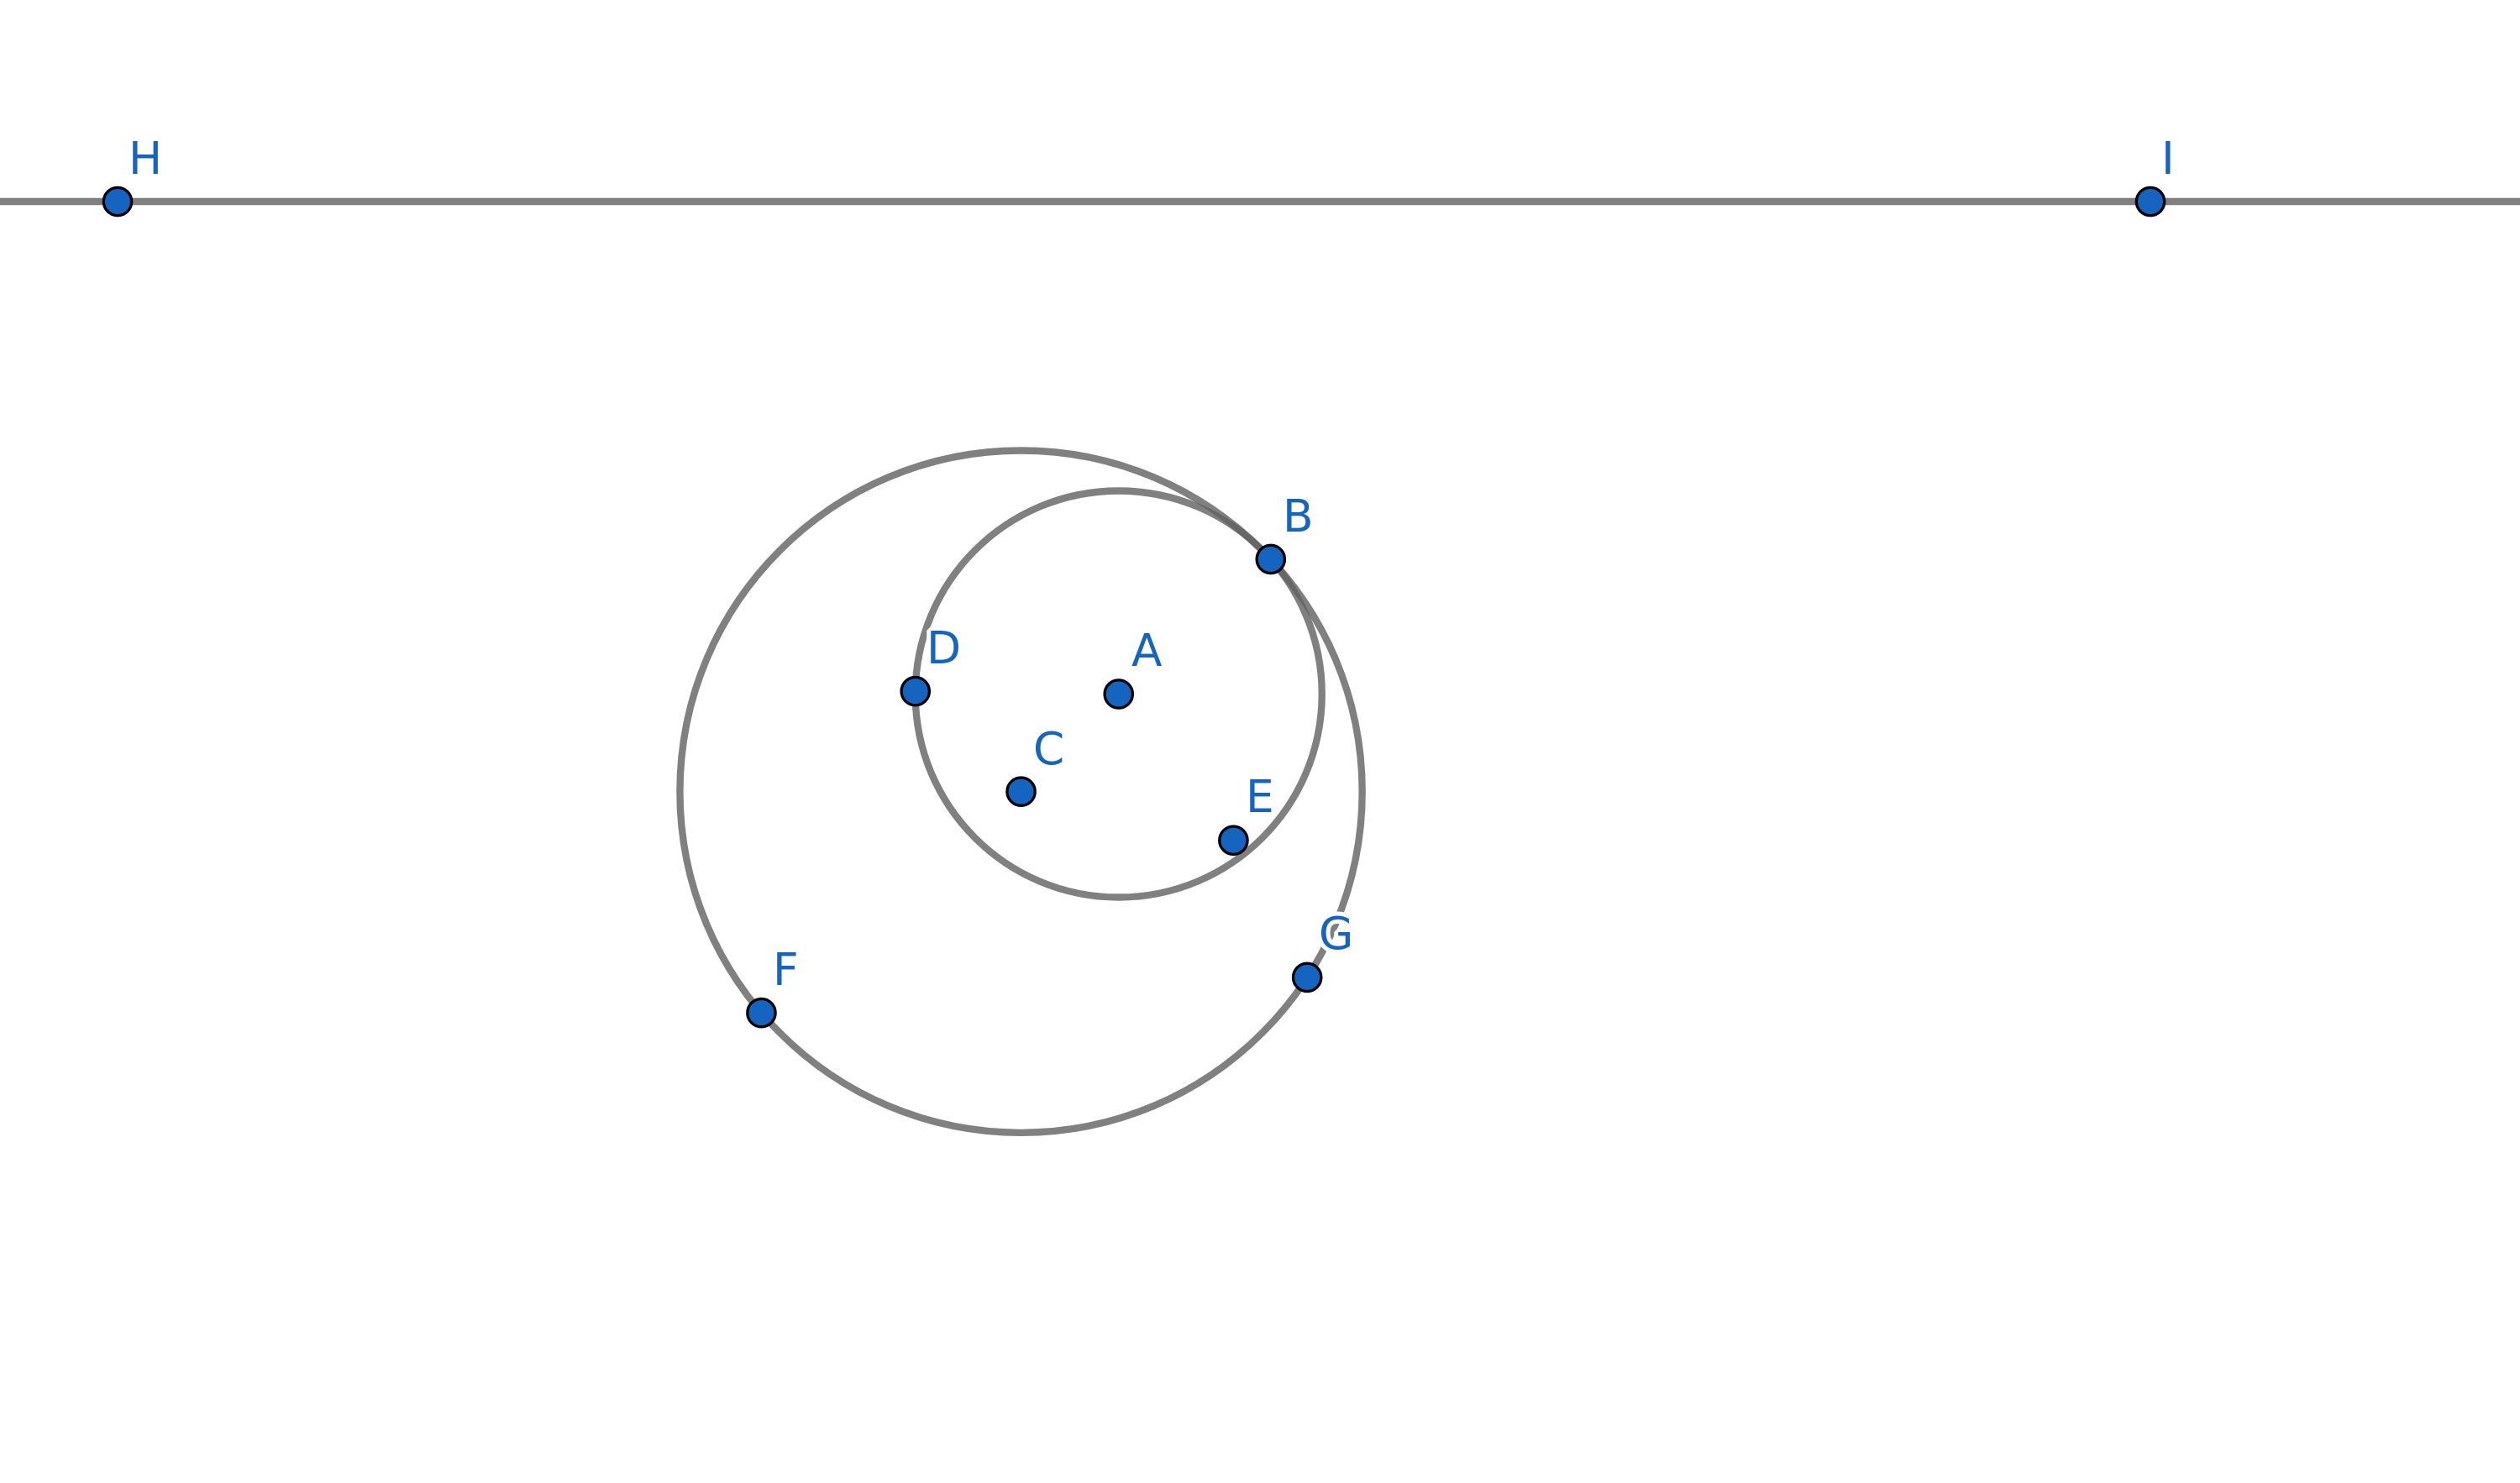
\includegraphics{circle-event.png}
                    \caption{circle events}
                    \label{fig:my_label}
                \end{figure}
                \end{displayquote}
                
            \item moving the  {\it{sweepline}}  
              \begin{displayquote}
                How the three components will be affected
                \begin{itemize}
                    \item no event {\textit{event}} is encountered:
                    Update the intersection points and edges
                    \item {\textit{site event}} update intersection points:
                    \item {\textit{circle event}} 
                    
                \end{itemize}
                
              \end{displayquote}
            \end{itemize}
            \end{displayquote}
    \item overriding events 
   
   \subsubsection{{\color{black} Final}}
 
    \end{itemize}
    
\end{enumerate}

\section{Definitions}

\subsection{Cells} For any site, if the collection of edges that has the site as one of the focal points form a cycle. Also, each end of those edges are equidistant from three sites then this cell is convex and a valid Voronoi decomposition.

\textbf{Proof:}
    This cell is formed by an intersection of half-planes thus it's convex. Also, it's valid since if $a, b$ are equidistant from $p, q$ then the whole segment $[a, b]$ is equidistant  from $p, q$. %TODO add drawing
    
\section{Functions}
{\color{red} \tt - Go through all functions}
\subsection{Parabola Functions}
\subsubsection{Intersection of two arcs}
Let $p_1, p_2$ be two arcs and their intersections are $a_1, b_1$ then as the sweepline moves there will be new intersections $\left(a_1, b_1\right),\left(a_2, b_2\right),\dots \left(a_k, b_k\right)$ the line segments formed by $a_i$s lies on the same line similarly  $b_i$s satisfy the same property.

The main method is to show that a solution belongs to two curves which boils down to algebraic manipulations.

\subsection{Lines, Circles, and distances}
\section{Events}
We assume that the algorithm has processed n events. We would like to check if we have given a correct decomposition then preforming a site event or a circle event will preserve the correctness of the decomposition up to the cliff.

\subsection{Bound on events length} If the beach-line is of length after a site event then at most there will be $n-2$ circle events. Thus, the queue length can't exceed $n^2$ where is the number of sites. Tightening this bound has no almost effect on the performance as it sole role to tell Coq the main function's recursion will terminate.



\end{document}